\section{Preliminary models}\label{Section:PreliminaryModels}

This section is divided into three subsections, one for each of the three use-case providers. Each of these sections begins with a subsection explaining state-of-the-art for the various application scenarios defined in Deliverable
1.2. In order to address the different application scenarios within the AMIDST project, use case-specific probabilistic graphical
models classes are designed. These model classes will, in turn, form the basis for the general AMIDST model class. Finally, we include discussions and
directions for possible further model extensions for each of the use case providers.  



% This section is divided into three subsections, one for each of the three use-case providers. Each of these sections, in turn,  begins with a subsection explaining the state-of-the-art for the various applications scenarios defined in Deliverable 1.2; another subsection is then added for each application scenario (that is, two subsections for Daimler and Cajamar and three for Verdande), which includes the probabilistic graphical models designed for that particular application scenario; finally, another subsection is included at the end of each use-case provider with further discussion and future models.

%-----------------------------------------------------------------------------------------------------------------------
\subsection{Daimler models}\label{Section:DaimlerModels}
%-----------------------------------------------------------------------------------------------------------------------

%-----------------------------------------------------------------------------------------------------------------------
\subsubsection{State-of-the-art of the application scenarios}\label{Section:StateOfTheArt}
%-----------------------------------------------------------------------------------------------------------------------

As has been described in Deliverable 1.2 \cite{Fer14b}, the Daimler use-case is based on two application scenarios: i) early recognition of a lane change manoeuvre; and ii) earlier prediction of the need for a lane change based on the relative dynamics between two vehicles driving in the same lane at different speeds. 

The first scenario has previously been addressed by Daimler \cite{Kasper2011,kasper2012object,KasperThesis2013}. The main result of this previous work was a static object-oriented Bayesian network (OOBN) \cite{KollerPfeffer1997} able to detect a manoeuvre 0.6 seconds before execution. The goal now is to enhance the prediction horizon for manoeuvre recognition by at least 1-2 seconds before execution, in order to further improve the quality of the on-board adaptive cruise control. 

As it will be explained later, this manoeuvre recognition improvement is expected to be achieved by introducing a dynamic extension of the previously proposed static OOBN model. We basically consider such a dynamic extension for two main reasons: First, although its limited prediction horizon, the static OOBN model has proven to be very robust for this task and it is considered as the gold-standard solution in Daimler. Second, AMIDST models are expected to be integrated in an electronic control unit (ECU) \cite{Fer14}, and we expect that the methods developed when integrating the static OOBN in this ECU \cite{Weidl2014} can also be exploited in the integration of this dynamic version. 

Note that, the basic setting of both application scenarios is as follows: Let us suppose we are driving our car, referred to as the EGO vehicle, on a highway. The EGO vehicle is equipped with a video camera, radar, and some on-board sensors. Using the data provided by these sensors, the challenge consists in making an early recognition of a manoeuvre either by the EGO or any other relevant car in the traffic scene referred to as Object vehicle (OBJ). In total, the system is expected to recognise the following set of manoeuvres (a visual description of them is given in Figure \ref{Figure:DaimlerManeuvers}):

\begin{figure}[ht!]
\begin{center}
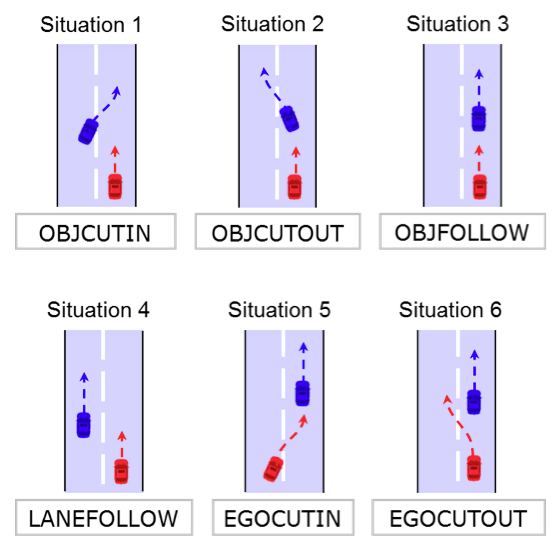
\includegraphics[scale=0.4]{./figures/DaimlerManeuvers}
\caption{\label{Figure:DaimlerManeuvers}The different manoeuvres to be identified by the AMIDST system. Red blocks represent the EGO vehicle while blue ones represent the OBJ vehicle.}
\end{center}
\end{figure}

\begin{enumerate}
\item \textbf{OBJ-CutIn}: The OBJ vehicle is moving to the lane where the EGO vehicle is placed.
\item \textbf{OBJ-CutOut}: The OBJ vehicle, which was driving in front of the EGO vehicle, is leaving now the EGO's lane.
\item \textbf{OBJ-Follow}: There is no lane change. The EGO is driving and there is another vehicle (i.e., OBJ) in front.
\item \textbf{LANE-Follow}: There is no lane change. The EGO is driving and there is no other vehicle in front.
\item \textbf{EGO-CutIn}: The EGO vehicle is moving right-direction to a new lane already occupied by another vehicle. 
\item \textbf{EGO-CutOut}: The EGO vehicle is leaving left-direction the lane where it was driving.
\end{enumerate}

Moreover, instead of working directly with the raw data from the video, radar, and on-board sensors, the current manoeuvre recognition system uses the so-called ``object data'', which contains ``high level'' representations or features describing the traffic scene such as EGO's speed, distance between EGO and another vehicle in front, etc. This is the data to be used for learning the OOBN models.

Figure \ref{Figure:DaimlerDataFlow} contains a visual description of the current data flow used to create the ``object data''.  First, the raw data coming from the video, radar, and sensors are preprocessed. Then, the preprocessed data is merged, and the high-level or ``object data'' describing the traffic scene is obtained. 

\begin{figure}[ht!]
\begin{center}
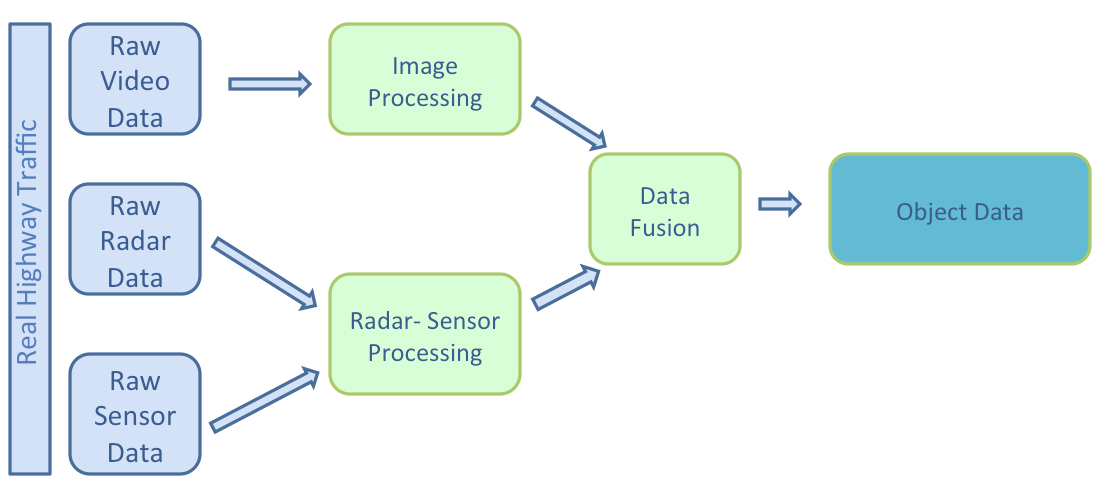
\includegraphics[scale=0.35]{./figures/DaimlerDataFlow}
\caption{\label{Figure:DaimlerDataFlow} Daimler's data flow.}
\end{center}
\end{figure}

In the following sections, we will introduce the Daimler models considered for both application scenarios.

%-----------------------------------------------------------------------------------------------------------------------
\subsubsection{Early recognition of a lane change manoeuvre}\label{Section:Daimler:EarlyRecognition}
%-----------------------------------------------------------------------------------------------------------------------

As commented above, Daimler has developed a static OOBN which is able to recognise an ongoing manoeuvre around 0.6 seconds before it really takes place \cite{kasper2012object}.  This model is partly described in the following section. But full details will be given in the confidential Deliverable 6.1.   

%-----------------------------------------------------------------------------------------------------------------------
\subsubsection*{Static OOBN model}
%-----------------------------------------------------------------------------------------------------------------------

This model works with the previously presented ``object data''. This data mainly consists of a set of measured and/or computed signals or situation-features denoted by $S$ (e.g., EGO speed, EGO lateral velocity, speed of car in-front, etc., see \cite{kasper2012object} for further details) describing the traffic scene. The situation features used for manoeuvre recognition are structured along three main dimensions: lateral evidence (LE), trajectory (TRAJ), and occupancy schedule grid (OCCGRID).  

Figure \ref{Figure:DaimlerSituationFeatures} shows a visual description of LE, TRAJ, and OCCGRID. They are referred to as the three possible hypotheses of a lane change manoeuvre: 1) LE hypothesis considers the lateral offset and the lateral velocity of a car and accounts for its lateral movement; 2) TRAJ hypothesis accounts for the evidence about a car's trajectory, measured by the car angle and the estimated time to cross the line; and 3) OCCGRID hypothesis accounts for the area surrounding a car and allows to detect if some other vehicle is moving to its adjacent environments.

\begin{figure}[ht!]
\begin{center}
\begin{tabular}{ccc}
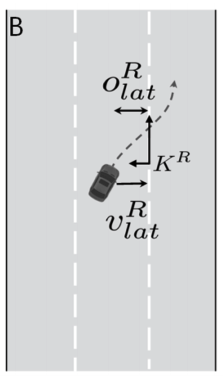
\includegraphics[width=2cm]{./figures/DaimlerLEHipothesis} &

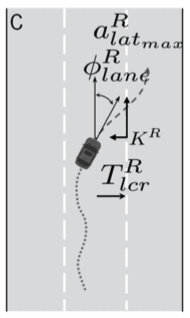
\includegraphics[width=2cm]{./figures/DaimlerTRAJHipothesis} &

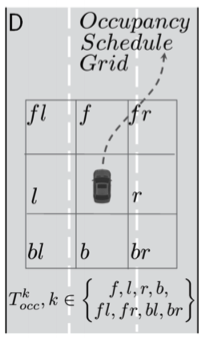
\includegraphics[width=2cm]{./figures/DaimlerOCCGRIDHipothesis} \\

Lateral evidence & Trajectory & Occupancy grid \\
\end{tabular}
\caption{\label{Figure:DaimlerSituationFeatures} The three main dimensions of the situation features \cite{kasper2012object}.}
\end{center}
\end{figure}

The general structure of this OOBN model consists of a number of abstraction levels as detailed in Figure \ref{Figure:DaimlerOOBNAbstraction}: 

\begin{itemize}
\item \textbf{Class S: Sensor measurement}: This class represents objects at the lowest level of the OOBN. It models the so-called \textit{measured data}, which consists of a set of observations, acquired from sensors and computations, characterising situations in the traffic scene. The general structure could be considered as a standard noisy sensor model \cite{JensenNielsen2007}, where S\_MEAS refers to the sensor-reading value, S\_REAL refers to the real value and S\_SIGMA refers to the uncertainty in the measurements. As it can be seen, S\_MEAS is conditionally dependent on the random changes in S\_REAL as well as the sensor noise/fault (S\_SIGMA). In Daimler, the observations of the measured value S\_MEAS and the uncertainty of the measurement S\_SIGMA are given in the object data. 

\item \textbf{Class H: Hypothesis}: This class pertains to a higher level and directly depends on the real values S\_REAL obtained in the previous class. In fact, the real sensor values are used to evaluate the different possible hypotheses namely LE, TRAJ and OCCGRID. 

\item \textbf{Class E: Event}: This class is at the top level of the modelling. It allows to model a high-level Hypothesis/Event based on a set of low-level hypotheses ($Hypothesis_1, \ldots, Hypothesis_n$) in a recursive way. This class also includes the \textit{Event} variable representing the possible traffic manoeuvres of the EGO and OBJ vehicles. 

\end{itemize}

\begin{figure}[ht!]
\begin{center}
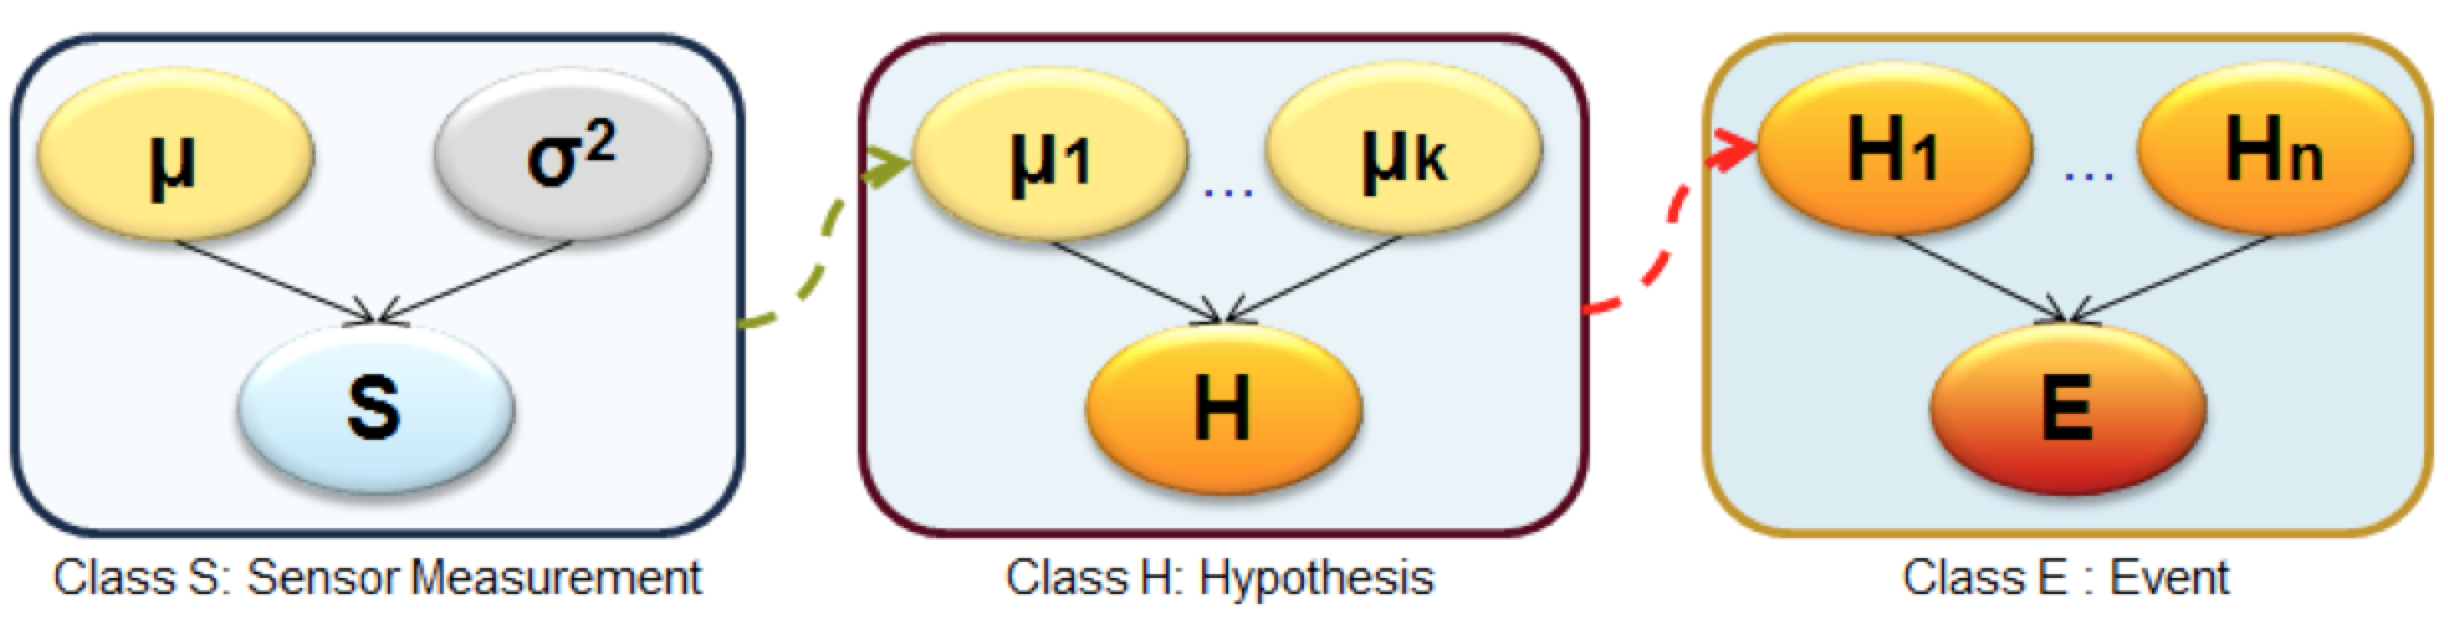
\includegraphics[scale=0.48]{./figures/DaimlerOOBNAbstraction}
\caption{\label{Figure:DaimlerOOBNAbstraction} The static OOBN model used to predict an event \cite{Weidl2014}.}
\end{center}
\end{figure}

Finally, Figure \ref{Figure:DaimlerLE} shows a concrete fragment of the static OOBN model related to the LE hypothesis modelling. As it can be seen, LE hypothesis depends on the lateral offset to a lane marking, O\_LAT\_REAL, as well as on the lateral velocity, V\_LAT\_REAL, of the car. Both measures are estimated from their measured values, O\_LAT\_MEAS and V\_LAT\_MEAS, respectively, and from the estimated uncertainty of the measurements, O\_LAT\_SIGMA and V\_LAT\_SIGMA. This OOBN fragment is used to model the growing probability for LE to cross the lane marking, based on the vehicle coming closer to the lane marking and the increase of its lateral velocity.

\begin{figure}[ht!]
\begin{center}
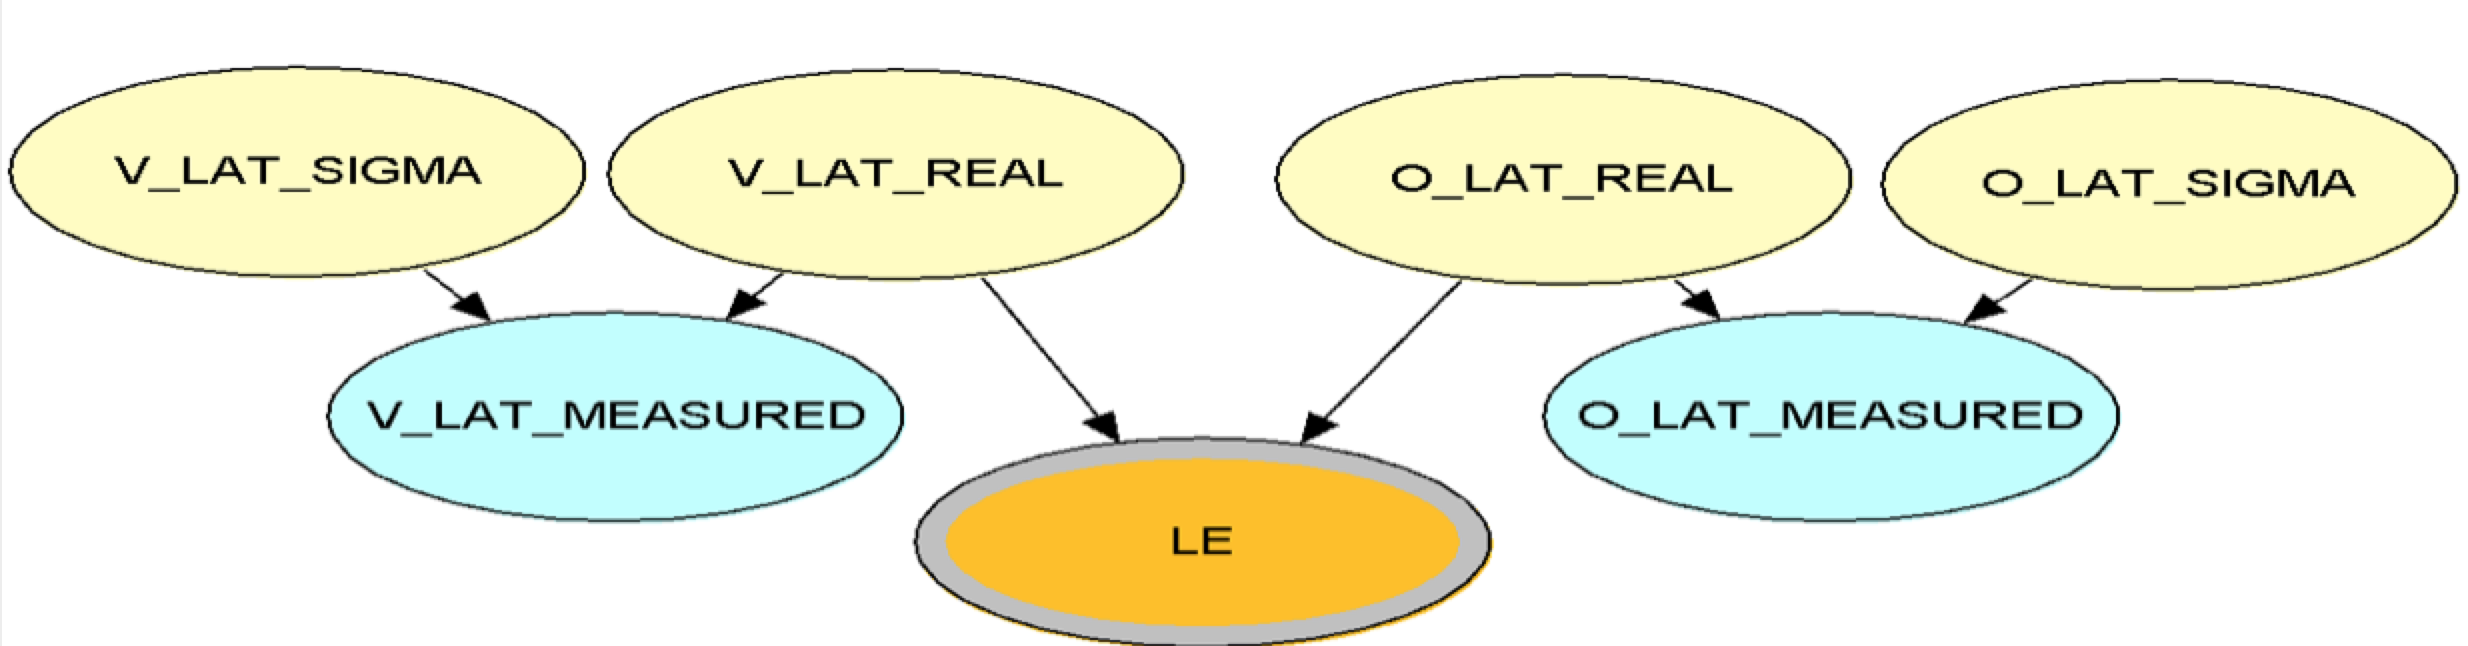
\includegraphics[scale=0.48]{./figures/DaimlerLE}
\caption{\label{Figure:DaimlerLE} Static-OOBN fragment for the lateral evidence hypothesis.}
\end{center}
\end{figure}

Note that, the static OOBN model contains both continuous and discrete variables. It was parametrized using the CLG framework\cite{JensenNielsen2007,lauritzen1996graphical} that allows continuous children with continuous parents and multinomial distributions for discrete children with discrete parents. In addition, we have discrete children with continuous parents (i.e., the low-level Hypothesis depending on S\_REAL$_1$, \ldots, S\_REAL$_k$ variables) that were initially parametrized using a logistic function. However, as discussed in Section \ref{Section:Preliminaries}, this modelling has a significant impact when making inference. A possible solution used in \cite{kasper2012object} is to discretize S\_REAL variables. Given that S\_MEAS and S\_SIGMA are always observed, their potentials can be therefore collapsed/combined with the potential of the corresponding discretized S\_REAL variables. Consequently, all the inferences in the resulting model can be performed using only discrete potentials \cite{JensenNielsen2007}.
